\documentclass[openright,twoside,10pt]{book}
\usepackage[b5paper,left=2cm,top=2.5cm,right=1.5cm,bottom=2.5cm]{geometry} 
\usepackage[spanish]{babel} % espanol
\usepackage[utf8]{inputenc} % acentos sin codigo
\usepackage{graphicx} % gráficos
\usepackage{lscape}
\usepackage{fancyvrb}
\usepackage{fancyhdr}
\usepackage{wrapfig}
\setlength{\parskip}{10pt plus 1pt minus 1pt}
 % aqui definimos el encabezado de las paginas pares e impares.
\rhead[]{}

\renewcommand{\headrulewidth}{0.5pt}

% aqui definimos el pie de pagina de las paginas pares e impares.
\rfoot[\thepage]{\thepage}
\cfoot[]{}
\renewcommand{\footrulewidth}{0pt}

%redefino el verbatim
%\renewenvironment{verbatim}{\begin{Verbatim}[frame=single,fontsize=\small]}{\end{Verbatim}}


% aqui definimos el encabezado y pie de pagina de la pagina inicial de un capitulo.
\fancypagestyle{plain}{
\fancyhead[R]{}
\fancyfoot[C]{}
\fancyfoot[R]{\thepage}
\renewcommand{\headrulewidth}{0.5pt}
\renewcommand{\footrulewidth}{0pt}
}

\pagestyle{fancy} % seleccionamos un estilo



\date{21 de Enero de 2020}
\author{Velasco Gil, Álvaro}

\title{TFG: titulo}

\begin{document}

\begin{titlepage}

\begin{center}
\vspace*{-1in}
\begin{figure}[htb]
\begin{center}
\includegraphics[width=3cm]{./img/logo}
\end{center}
\end{figure}
\begin{large}
\textbf{Universidad de Valladolid}
\end{large}

\vspace*{0.15in}

\vspace*{0.6in}
\begin{large}
\textbf{ESCUELA DE INGENIERÍA INFORMÁTICA}

\end{large}
\vspace*{0.2in}
\textbf{ GRADO EN INGENIERÍA INFORMÁTICA}\\
\textbf{ MENCIÓN EN INGENIERÍA DEL SOFTWARE }
\vspace*{0.1in}
\rule{140mm}{0.1mm}\\
\vspace*{0.2in}
\begin{large}
\textbf{{\LARGE DISEÑO E IMPLEMENTACIÓN DE UN SISTEMA DE CONTROL Y MONITORIZACIÓN DE ASISTENTES INTELIGENTES\\}}
\end{large}
\vspace*{0.2in}
\rule{140mm}{0.1mm}\\
\vspace*{2in}
\begin{large}
\begin{flushright}
\textbf{Alumno: Velasco Gil, Álvaro \\
\vspace*{0.3in}
Tutor: Vegas, Jesús }
\end{flushright}
\end{large}
\end{center}

\end{titlepage}

\newpage
\mbox{}	
\thispagestyle{empty} % para que no se numere esta página

\chapter*{}
\pagenumbering{Roman} % para comenzar la numeración de paginas en números romanos
\begin{flushright}
\textit{%Dedicatoria,\\
Pequeña dedicatoria.}
\end{flushright}

\chapter*{Agradecimientos} % si no queremos que añada la palabra "Capitulo"
\addcontentsline{toc}{chapter}{Agradecimientos} % si queremos que aparezca en el índice
\markboth{AGRADECIMIENTOS}{AGRADECIMIENTOS} % encabezado 

% Aquí agradecer

\chapter*{Resumen} % si no queremos que añada la palabra "Capitulo"
\addcontentsline{toc}{chapter}{Resumen} % si queremos que aparezca en el índice
\markboth{RESUMEN}{RESUMEN} % encabezado
\begin{flushleft}

El fin de este proyecto es el de crear un sistema capaz de monitorizar y controlar remotamente diferentes dispositivos que serán utilizados como asistentes inteligentes.

Para el desarrollo de este proyecto se ha utilizado diferentes lenguajes, como Kotlin en el backend, Python en los dispositivos, y VueJS, HTML y CSS en el frontend, siguiendo un plan basado en iteraciones.

% Aquí el resumen

\end{flushleft}

\chapter*{Abstract} % si no queremos que añada la palabra "Capitulo"
\addcontentsline{toc}{chapter}{Abstract} % si queremos que aparezca en el índice
\markboth{ABSTRACT}{ABSTRACT} % encabezado
\begin{flushleft}

% Aquí va el abstract

\end{flushleft}

\tableofcontents % indice de contenidos

\cleardoublepage
\addcontentsline{toc}{chapter}{Lista de figuras} % para que aparezca en el indice de contenidos
\listoffigures % indice de figuras

Aquí aparecerá la lista de imagenes que hay en el TFG

\cleardoublepage
\addcontentsline{toc}{chapter}{Lista de tablas} % para que aparezca en el indice de contenidos
\listoftables % indice de tablas

Aquí aparecerá la lista de tablas que hay en el TFG

\chapter{Introducción}\label{cap.introduccion}
\pagenumbering{arabic} % para empezar la numeración con números
\section{Introducción}

En este proyecto se abordará el proceso de control y monitorización remota de dispositivos asistentes inteligentes.

Tras la lectura de este documento se comprenderán tanto los motivos por los cuales se ha decidido tomar esta opción, como el proceso de despliegue del sistema, pasando por las fases de implementación en las que se enseñará a replicar proyectos de estructura similiar, como por las fases de desarrollo en la cuales se estudian los posibles riesgos y carácterísticas del proyecto, al igual que por el plan de desarrollo en el que se programa toda la elaboración.

\section{Motivación}

Los asistentes inteligentes están en auge y las grandes empresas están dando acceso a estos servicios de manera gratuita, donde lo único que hay que hacer para disfrutar de ellos es pagar es el dispositivo físico, en caso de que se requiera, lo que hace cuestionar la idea del modelo de negocio que están siguiendo para que salga rentable.

Este modelo de negocio hace pensar que el producto en realidad es cada usuario que lo utiliza, del que están recopilando información. Esta información al ser obtenida directamente de los hogares de cada usuario no es solamente privada, si no que también es íntima, lo que hace cuestionarse si realmente la comunidad de usuarios sabe que hay empresas aprovechándose de su día a día para recolectar toda la información mediante esos dispositivos que, situados en los lugares más personales de cada usuario, capturan información con gran potencial, ya sea sobre gustos, tendencias, necesidades o inclinaciones políticas, pudiendo todos estos datos estar siendo vendidos, o utilizados por terceros.

Esta ignorancia global sobre el tratamiento de los datos obtenidos por el dispositivo hace replantear la posibilidad de creacción de un nuevo dispositivo asistente, el cual haga más facil la vida de un sesgo de la sociedad al cual iría orientado, sin tener la necesidad ni posibilidad de almacenar datos de carácter sensible.

Por otro lado, la despoblación y migración por la parte joven de la sociedad está provocando una despobación en sus lugares de origen, dejando a los familiares de mayor edad en soledad, siendo la parte de la familia que a grosso modo necesita más atención y requiere más ayuda para pasar el día.

La implementación de un asistente inteligente el cual ayude a este conjunto de la sociedad a entretenerse proponiendo tanto eventos cercanos a ellos, como respondiendo sus dudas de una manera rápida, o sirviéndoles para buscar ayuda en caso de posible caída o solicitud de auxilio, puede ser una gran herramienta que mejore sus calidades de vida.


\section{Objetivos}

El objetivo de este proyecto es, por tanto,xs el despliegue de un sistema que permita la conexión de dispositivos asistentes al servidor de manera automática y remota, pudiendo ser controlados desde una web de administración, al igual que pudiendo ver estadísticas de uso para comprobar el estado de los usuarios. 

Estos dispositivos estarán orientados a personas de la tercera edad, estando asignado cada dispositivo a una persona, y conteniendo entonces información relacionada con la localidad a la hora de responder.

Los dispositivos podrán entonces ser controlados y configurados de manera individual, en función de su localidad, o de una manera global, pudiendo enviar actualizaciones a través de configuraciones, al igual que mandar la realización de diferentes acciones.


\chapter{Estado del arte}\label{cap.arte}
\section{Introducción}
Los asistentes inteligentes están buscando su hueco en todo hogar, y esto es un hecho.
Estos asistentes nos hacen la vida más sencilla, ayudando a actualizar y controlar toda la domótica de nuestras casas con acciones que hace unos años solo podíamos imaginarlas en películas de ciencia ficción.

El concepto de asistentes de voz, que tan de moda está ahora entre la población joven, junto con la gente de edad avanzada que necesita interacción en sus vidas puede ser una combinación perfecta para ayudarles a no perder el contacto con la sociedad.

La creación de un asistente que pueda resolver sus dudas, con el que puedan hablar, al que puedan preguntar a qué hora es la partida de cartas en el bar, o al que puedan pedir auxilio en caso de una caída, puede ser de gran utilidad para mejorar su día a día, al igual que servir de alivio para el resto de familiares que no pueden estar cerca de sus seres queridos, sabiendo que van a poder ser informados rápidamente de un posible accidente.

Pero el auge de los dispositivos asistentes pone en vilo la gestión de la privacidad e intimidad que hay dentro de nuestras casas,n y todo esto es debido a que pueden recolectar información a través de escuchar las conversaciones de nuestro día a día, siendo información que no sabemos a dónde va a parar, qué se va a hacer con ella.

Esta información es de un caracter sensible, ya que puede contener desde nuestros simples gustos, incluyendo nuestras necesidades, hasta nuestras tendencias políticas, siendo datos que pueden estar siendo utilizados por terceros, o incluso siendo vendidos ante nuestro desconocimiento.

La falta de soluciones en el mercado que cumplan todos estos puntos suponen una motivación para la creación de un asistente que no esté conectado constantemente a internet, ya que las personas de edad avanzada seguramente no tengan contratado el servicio, y que tampoco almacene datos de carácter sensible de los usuarios, sino que simplemente interaccione con cada persona, y la ayude en su día a día, tanto ofreciendo actividades de la misma localidad, como respondiendo cualquier pregunta que pase por la cabeza de quien lo posea, al igual que buscando ayuda en caso de que una persona requiera auxilio.

Antes de adentrar en la elección de un asistente inteligente, se expondrá qué es, y cuál es su funcionamiento, para entender mejor los motivos por los cuales se acaba eligiendo uno en vez de otro.

\subsubsection{Qué es un asistente inteligente}

Un asistente inteligente es simplemente una máquina programada de manera que su comportamiento se asemeje al de una persona a la que se solicita asistencia, como su propio nombre indica, pudiendo mantener una conversación que siga los protocolos de comunicación humana.

\begin{figure}[h!]
    \centering
    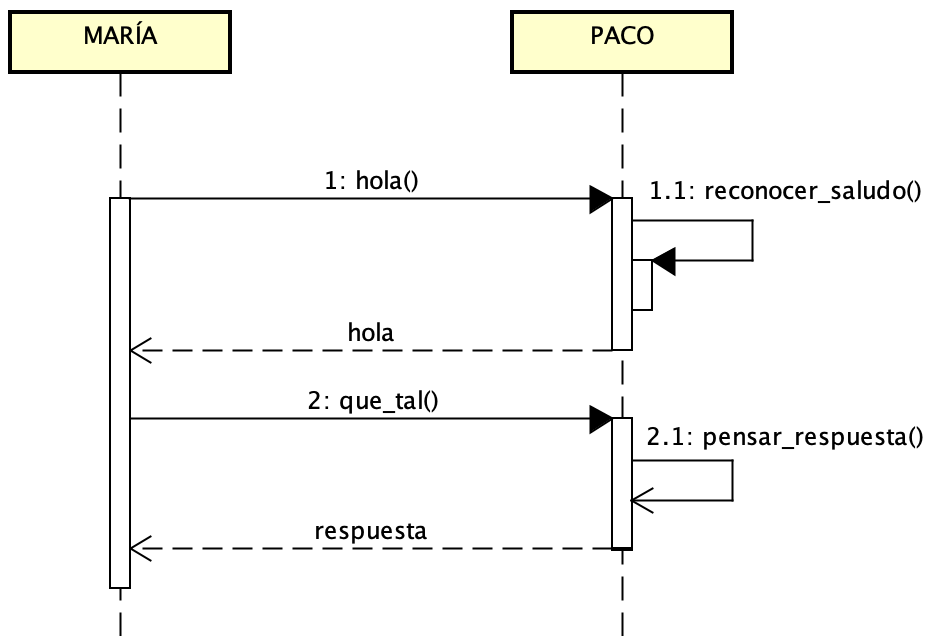
\includegraphics[width=10cm]{./img/sequence/human.png}
    \caption{Secuencia de comunicación humana}
    \label{fig:humanseq}
\end{figure}

Como se puede ver en la figura \ref{fig:humanseq}, un protocolo de comunicación entre dos personas se basaría en un saludo para entablar conversación, para posteriormente realizar una pregunta.

En el caso de los asistentes, el proceso de conversación se basa en lo mismo: un usuario saluda al asistente mediante el uso de una palabra o conjunto de palabras, al que se llamará \textbf{hotword}, que cuando sea reconocido por el asistente inteligente, devolverá el saludo.
Es entonces cuando el usuario debe realizar la pregunta o solicitar la información que requiera.
Una vez hecha la pregunta, el dispositivo se pondrá a pensar la posible respuesta, entrando en el proceso al que se llamará \textbf{reconocimiento de los hechos}. Una vez identificados los hechos, devolverá la respuesta que más se acerque a lo deseado, gracias a un entrenamiento previo.

\subsubsection{Cómo piensa el asistente}

El proceso de pensamiento analizado entre los principales asistentes, que se expondrá en este capítulo tiene una estructura similiar independientemente del tipo de asistente que se trate, asemejándose a la figura \ref{fig:humasseq}.

\begin{figure}[h!]
    \centering
    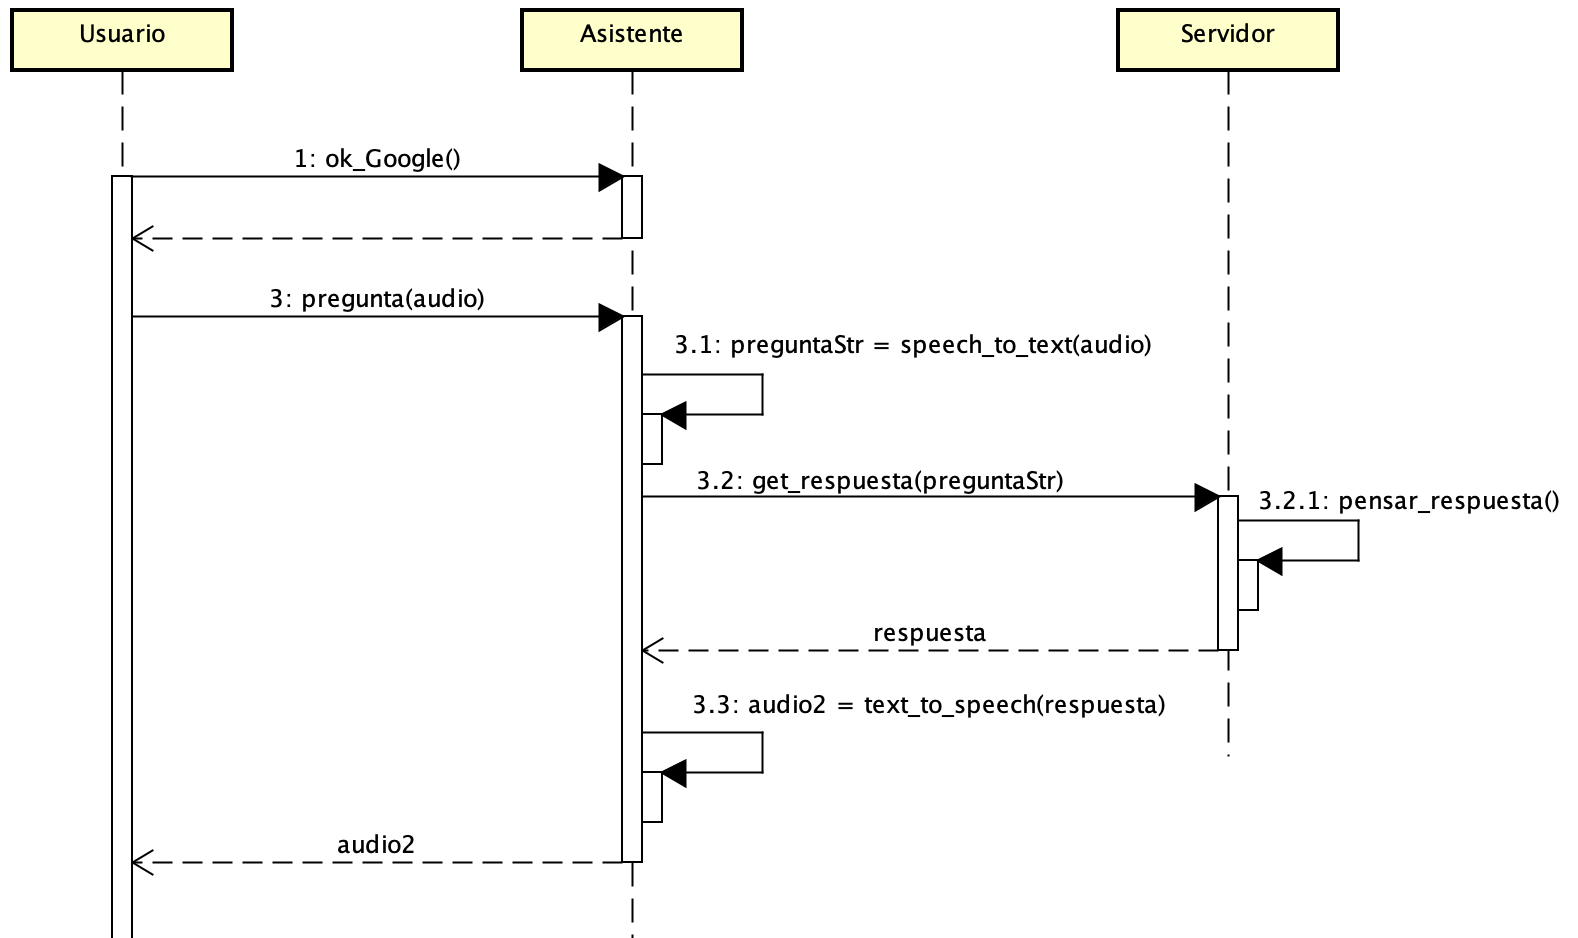
\includegraphics[width=14cm]{./img/sequence/humasseq.png}
    \caption{Secuencia de comunicación humano-asistente}
    \label{fig:humasseq}
\end{figure}

Lo que diferencia a un asistente de otro, es la manera en la cual piensa la respuesta, dando mayor validez a un asistente que dé una respuesta más aproximada a lo solicitado.
Para esto, la mayoría de asistentes tienen el procesamiento de la respuesta en la nube debido a la gran cantidad de información que tienen almacenada para contrastar los hechos capturados, al igual que también tienen en la nube el proceso de speech-to-text o el de text-to-speech.


\section{Requisitos mínimos}
Una vez que ya se ha expuesto cual es el funcionamiento base de un asistente virtual inteligente, interesa saber cual es que más se adecúa a las necesidades establecidas para este proyecto, de manera que se le exijirá que cumpla el máximo de los siguientes puntos expuestos.

\subsubsection{Despliegue en dispositivos}

El asistente seleccionado debe poder ser desplegado de manera gratuíta en un dispositivo formado por una placa RasbperryPi, o similar.

Para ello, se requiere que el asistente disponga de una librería o de un modo de uso que se pueda implementar en un dispositivo pequeño y portátil, facilitando el cambio de una ubicación física por otra de los distintos posibles lugares que existen dentro de un hogar, manteniendo una instalación lo más simple y limpia posible, en la que solo sea requerida la localización de un enchufe a la toma de la luz.

\subsubsection{Tratamiento de la información}

El asistente debe seguir la ley orgánica de protección de datos, y no debe tener acceso a escuchar conversaciones ajenas violando la intimidad de los usuarios.

Cualquier vacío legal o conjunto de cláusulas de extensa longitud no podrá será aceptado, para poder asegurar la protección de los datos de los usuarios.

En caso de almacenar algún tipo de dato, debe poder ser público para el usuario en cuestión, o haber sido aceptado expresamente por el usuario a favor de un control de su seguridad.

\subsubsection{Conexión a Internet}

La orientación de un dispositivo asistente inteligente como este a personas de una edad avanzada debe tener en cuenta que es posible que la mayoría de sus usuarios potenciales no tengan una conexión a internet en sus respectivos hogares.

Esto provoca que la conexión del dispositivo a la red tiene que ser lo mínima posible, favoreciendo los asistentes en los cuales el proceso de pensamiento sea ejecutado dentro del propio dispositivo, evitando tener que hacer el cálculo e identificación en servidores de alojados en la nube.

Es decir, el dispositivo debe ser capaz de funcionar en el lugar más remoto posible y sin ninguna conexión a internet, simplemente tras ser conectado a una red eléctrica.

\subsubsection{Adicción de nuevas tareas}

El software del asistente inteligente debe tener la capacidad de añadir nuevas tareas fácilmente, de modo que se puedan añadir nuevas funciones tanto propias, como desarrolladas por la comunidad de Internet.

\section{Mercado}
En los siguientes apartados se mostrarán las diferentes opciones que ofrece ya el mercado para el uso de asistentes inteligentes, con el fin de comprobar la existencia de alguno que ya tenga establecidos los requisitos base ya descritos, o que permita la opción de poder establecerlos.

    \subsection{Google Assistant}
    El asistente inteligente de Google es el que está en el año 2020 a la cabeza de los asistentes virtuales********ENLACE********, y esto es debido a que viene instalado en todos los dispositivos Android, ocupando estos dispositivos la mayor parte del mercado de la telefonía móvil. Esta posición privilegiada le da un mayor entrenamiento, elevando el acierto y usabilidad de este.

La creación de Google tiene una gran aceptación con los diferentes aparáticos de la domótica del hogar, facilitando la implementación y realización de tareas:

- Una tarea es un conjunto de acciones que se llevan a cabo tras accionarse un evento que hace de interruptor, pudiendo ser el evento tanto un comando de voz, la pulsación de un interruptor o la activación de un sensor, entre otras opciones.

De esta manera, Google permite el control de la domótica del hogar, o la realización de diferentes acciones en nuestro día a día, pero requiere ser configurado por cada usuario, evitando por tanto la posibilidad de un despliegue común.

\subsubsection{Cómo funciona}

El proceso de pensamiento que hace el asistente de Google está basado en la nube, pero no solo eso sino que Google hace en sus servidores también el proceso de Speech-to-Text.

De este modo, Google almacena todos los audios que se le mandan a través de su asistente, estudiándolos uno a uno y asegurando o corrigiendo sobre la respuesta que envió el asistente.

Este proceso de corregir o confirmar es el método que tiene Google de entrenamiento, de manera que en la próxima consulta sobre el mismo tema, el asistente pueda responder con mayor exactitud.

Queda claro que sobre la teoría es un buen plan de entrenamiento, y en un mundo ideal esto sería perfecto, pero esos audios también pueden contener parte de información privada, o pueden servir para espiar conversaciones privadas que un usuario puede no querer que estén almacenadas, ni que sean escuchadas por otra persona, aunque sea un propio trabajador.

https://elpais.com/tecnologia/2019/07/18/actualidad/1563466196_049167.html

En cuanto a la posibilidad de ser desplegado en otro dispositivo que no sea un smartphone o una tablet, Google nos lo pone fácil, ya que otorga una librería con la cuál facilita la instalación y uso en una gran variedad de dispositivos, cuyo requisito es que dispongan de conexión a Internet.


    
    \subsection{Amazon Echo}
    También conocido como Alexa, es la opción creada por Amazon que más fuerza está tomando en la sociedad para ser elegida como la asistente de voz inteligente que nos acompañe en nuestro día a día.

A pesar de todas las ventajas posibles similares a las que se han descrito para el asistente de Google, también comparte sus contras, como las referentes a la localización donde se procesan los audios y donde se efectúa el entrenamiento, por lo que es otra opción que va a ser rechazada.

Sin tener en cuenta la ubicación del proceso de penamiento, Amazon asegura que almacena todos los audios hasta que es el propio usuario quien decide borrarlos, pero aún con la solicitud expresa del usuario, no pueden ser borrados completamente ya que han sido compartidos con terceros, que son quienes han desarrollado funciones específicas, llamadas Skills, y que son ellos quien pueden tener los datos del usuario almacenados, sin que el propio Amazon sea capaz de borrarlos aunque quisiese.

https://www.elmundo.es/tecnologia/2019/07/04/5d1ccf42fc6c833f3f8b460d.html
    
    \subsection{Mycroft}\label{Microft}
    Ante la falta de privacidad por parte de Google y Amazon, se abre la puerta a Mycroft, proyecto open source que busca como pilar la seguridad de los datos y la protección de la privacidad, de manera que asegura no almacenar ningún dato o información del usuario potencial.

Mycroft tiene la mayor comunidad para el desarrollo e implementación de asistentes, de modo que dispone de una gran cantidad de skills que añadir a nuestro dispositivo, posicionándose como opción principal para la elaboración del proyecto.

Este asistente virtual puede ser fácilmente implementado en dispositivos tales como Raspberry, cumpliendo los propósitos y requisitos de este proyecto.

En cuanto a la conexión a Internet, el equipo de Mycroft informa acerca de estar trabajando en una herramienta que permita desplegar el asistente ya entrenado dentro del dispositivo, evitando la conexión, pero de momento esa herramienta no está finalizada, por lo que cojea en ese aspecto y de momento, debería tener una conexión permanente.

En caso de que estén en lo cierto y estén trabajando en esa herramienta, este asistente ocuparía la primera opción como asistente a desplegar, pero en el momento actual en el cual este proyecto cobra vida, no es viable su implementación.


    
    \subsection{Snips Seeed}
    Snips Seeed es una  plataforma de inteligencia artificial para el desarrollo de dispositivos asistentes.

Esta plataforma nos permite crear nuestro propio asistente basandose en un entrenamiento previo con unos hechos predefinidos por el desarrollador.

En ese entrenamiento previo, se permite al asistente tomar lo aprendido de otros skills, que son fácilmente añadibles.

Tras la implementación en el dispositivo físico, el asistente ya ha sido entrenado, por lo cual no necesita estar más conectado a internet, siendo este el mayor aunto a favor, ya que es la carencia del resto de asistentes.

En cuanto a su uso, el dispositivo solamente escucha el ambiente comprobando si recibe el \textit{hotword}. Este hotword puede ser modificado por cualquier otra palabra que se desee, lo cual beneficia a que en este proyecto se pueda asignar una palabra más acorde a las personas a quienes va orientado.

El asistente, en cuanto a su configuración interna, sigue el protocolo de comunicación descrito en la figura \ref{fig:humasseq}, con una pequeña modificación:
Cuando el servidor ya ha entendido la pregunta o solicitud, genera unos hechos definidos en su entrenamiento en forma de objecto, que envía el skill \textit{skill-server} a través de un puerto MQTT, y se queda a la espera de una respuesta.

Los otros skills, que han sido añadidos previamente en el entrenamiento, están levantados escuchando por el puerto, de manera que identifican los objectos que circulan por él y comprueban si ese hecho le corresponde, que de no ser así, simplemente lo ignora.
Una vez que un skill captura un hecho que sí que le corresponde, comprueba los \textit{slots} que contiene dicho hecho para ver qué es lo que se está solicitando. Tras esto, genera una respuesta en forma de cadena de texto, y la envía por el puerto MQTT para que la recoja el \textit{skill-server}.

Una vez capturada por este, simplemente transcribe el mensaje a audio con su skill de text-to-speech, y se lo transmite al usuario a través del altavoz, finalizando la comunicación.

Como se puede ver, el tratamiento de la información que se le otorga al dispositivo es el que nosotros deseemos, ya que el asistente no envia nada al exterior. De esta manera, nosotros controlamos qué sucede con la información, siendo el otro punto requerido en la búsqueda de un asistente ideal.

Como extra, Snips Seeed es una plataforma gratuita que se basa en una colaboración de una gran comunidad de desarrolladores. Pese a ser esta comunidad de menor tamaño que la conseguida por la opción de Mycroft, hay una gran cantidad de aplicaciones disponibles como juegos, la consulta del tiempo o la consulta de noticias, preparadas para ser asignadas directamente a nuestro dispositivo.

Como se puede ver, SnipsSeeed otorga las herramientas necesarias para cumplir todos los requisitos estipulados anteriormente, siendo la plataforma que se pone a la cabeza como posible elección.

    
    \subsection{Elección final}

La elección más acorde de entre todas las propuestas es el uso Snips Seeed, ya que se adapta a todos nuestros requisitos.

En cuanto al proyecto, va a ser necesario el desarrollo de un dispositivo que contenga este asistente, al igual que el diseño y desarrollo de un backend capaz de albergar la información relativa a cada dispositivo.

Para la gestión de estos dispositivos también será necesaria la implementación de una página web, desde la cual puedan ser los dispositivos configurados, manejados y controlados.

La implementación operativa de todo este sistema formaría un proyecto de gran embergadura, por lo que en los siguientes capitulos se documentará el diseño y desarrollo del backend y del frontend, mostrando el control y gestión real de un dispositivo el cual su rango de funciones será breve, de modo que se establezca la base y se explique como puedan ser añadidas nuevas funciones de una manera simple y sencilla.

NOTA: A fecha de 31 de Enero de 2020, Snips Seeed ha sido comprada por la compañía Sonos, privatizando las funciones y el acceso a entrenamientos de nuestro asistente. Este riesgo no se pudo preveer ya que se analizó un posible modelo de negocio interno de la compañía que le daría fuerza para ponerse como potencia en el mundo de los asistentes virtuales, ya que era el único capaz de evitar la conexión a Internet. Sonos vió también esa capacidad y quiso comprarla para no compartirla y asi tener una buena baza para posicionarse en los próximos años como uno de los principales asistentes del mercado.


\chapter{Análisis del proyecto}\label{cap.analisis}
\section{Introducción}

\section{Requisitos}
\subsection{Funcionales}
\subsection{No funcionales}

\section{Riesgos}



\chapter{Plan de desarrollo}\label{cap.desarrollo}
\section{Introducción}
En el siguiente capítulo se mostrará cual ha sido el método por el cual se ha desarrollado el proyecto, al igual que se definirán las fases del plan de desarrollo a seguir.

También se mostrará y explicará cuales han sido tanto las herramientas utilizas, como las librerías necesarias para una correcta implementación y desarrollo del proyecto con el fin de acercar al lector a entender cómo se ha diseñado, y qué es lo necesario para poder replicar el contenido del mismo en otros proyectos similares.



\section{Metodología}
Para el desarrollo de este proyecto se ha escogido una implementación siguiendo la combinación de un modelo iterativo y un modelo incremental.****enlace

Este método puede describirse de una manera simple y rápida, basada en la repeticion de ciclos en los cuales se van mejorando las funcionalidades implementadas a partir de la experiencia del usuario, y añadiendo nuevas.

Cada ciclo puede describirse como la continuación de los siguientes pasos:

\begin{enumerate}
    \item El desarrollador muestra un prototipo.
    \item El usuario lo prueba.
    \item El usuario muestra su experiencia tanto positiva como negativa, comentando posibles mejoras y proponiendo nuevas funcionalidades.
    \item Se subsanan esas carencias.
    \item Se obtiene una nueva versión del prototipo.
    \item Vuelta al paso inicial.
\end{enumerate}{}

La elección de este modelo se debe, por tanto, a la naturaleza del proyecto del cual se trata: al estar trabajando con unas nuevas tecnologías, y no tener muy claras las capacidades de las cuales los posibles asistentes están dotados, es preferible realizar un desarrollo basado en la entrega de pequeños prototipos que nos vayan ampliando el conocimiento de todas las posibilidades que van a poder ser implementadas, al igual que produce una retroalimentación a partir de la experiencia del usuario, siendo bastante útil tanto para mejorar, como para eliminar o para añadir nuevas funcionalidades.

En el caso del presente proyecto, el usuario el cual realiza las pruebas del prototipo se trata del propio tutor del proyecto, el cual otorga su experiencia, experiencia que está curtida a través de años de trabajo y perfeccionamiento, siendo más sabia que la del propio desarrollador, ayudando a elaborar un rediseño de las características que aumente la usabilidad. 

\section{Planificacion}
\label{planificacion}

\

Una vez conocido el método de trabajo que se seguirá para el desarrollo del proyecto, se deben conocer los plazos en los cuales el proyecto debe ser finalizado y entregado.

La fecha de inicio del proyecto es, por tanto, \textit{el 15 de Octubre de 2019}, y la fecha límite en la cual el proyecto debe ser entregado data del \textit{29 de Febrero de 2020}.

\subsubsection{Disponibilidad del desarrollador}

El proyecto se debe ajustar a una extensión de 300 horas, como fué especificado en el cálculo de costes en el apartado \ref{duracion_proyecto} del presente documento.

En cuanto a la disponibilidad del proyecto, el desarrollador carece de suficiente tiempo  al día como para elaborar 8 horas díarias, asemejándose a un trabajo real, debido a tener que compaginar las 7 horas diarias de un trabajo externo, con las necesarias para la completitud de dos asignaturas de la Universidad, y el presente proyecto.

Tras una planificación semanal, el desarrollador es capaz de asignar una media de 18.75 horas semanales, lo que supondría poder finalizar el proyecto en:

\begin{center}
    \textit{18.75horas/semana / 7 dias/semana = 2,67horas/dia }
    
    \textit{300horas / 2,67horas/dia = 112,5 días }  

\end{center}

\subsubsection{Organización de prototipos}

De este modo tras los cálculos anteriores, el proyecto sería finalizado aproximadamente 113 días después del inicio de este, datando de una fecha de finalización prevista para el día \textit{4 de Febrero de 2020}, teniendo una ventana para el posible retraso del proyecto de 25 días.

En cuanto a la planificación de las tareas, se contempla la posibilidad de entregar prototipos al usuario cada dos semanas, de este modo la planificación final constará de: 

    \begin{center}
    \textit{300horas/TFG / 18,75horas/semana = 16 semanas/TFG }
    
    \textit{ 16semanas / 2semanas/ciclo = 8 ciclos}
    \end{center}{}

Como consecuencia, el proyecto deberá ser realizado tras la iteración de 8 ciclos, obteniendo un prototipo en la finalización de cada iteración, resultando un total de 8 prototipos.


\section{Recursos y herramientas}
Para una correcta implementación que se adecúe a los requisitos, al igual que para un futuro manteniemiento del proyecto, enumerarán a continuación las herramientas que han sido utilizadas durante su desarrollo, con el fin de poder replicar en un futuro el entorno de trabajo en un futuro, o poder entender mejor cómo ha sido implementado.

    \subsection{Kotlin}

Kotlin es un lenguaje de programación funcional desarrollado por el equipo ruso de JetBrains como una evolución a Java por excelencia, permitiendo una interoperabilidad entre ambos, utilizándose bajo la JVM*******.

La sintaxis de Kotlin lo hace más intuitivo y simple, llegando al mismo resultado que en Java pero en un menor número de líneas, ahorrando tiempo y espacio.

Pese a que su gran popularidad es por el desarrollo Android, ahora está creciendo en su utilización en el lado del servidor gracias al framework de Ktor. 

    \subsection{Ktor}

Es un framework que se aprovecha de la usabilidad de Kotlin para el desarrollo de clientes y servidores asíncronos en la implementación de sistemas conectados.
Este framework será añadido al proyecto a través de la instalación de sus dependencias en gradle a través del fichero \textit{./build.gradle}.

    \subsection{Koin DI}
    \label{Koin}

Koin es un inyector de dependencias compatible con Kotlin, siendo bastante util para poder aplicar el principio de inversión de dependencias en el desarrollo del backend. 

La configuración de este inyector de dependencias es bastante simple, teniendo una sintaxis sencilla y útil en la que únicamente hay que utilizar Kotlin, evitando así los ficheros de configuración en XML que obligan a usar otros tipos de inyectores.

La utilización de este framework será util para poder aislar los casos de uso del sistema, de modo que no tengan dependencia de ninguna otra clase u servicio externo a los casos de uso, aumentando la escalabilidad del sistema y permitiendo una extensibilidad de los casos de uso en un futuro.

Para su utilización, se añaden las dependencias al fichero \textit{./build.gradle}.

Se implementará a través de la instalación de su módulo en el main de la aplicación.
\begin{lstlisting}
    // Declare Koin
    install(Koin) {
        modules(myModule)
    }
\end{lstlisting}

y en el módulo de Koin se indicarán los servicios que serán inyectados.
\begin{lstlisting}
// app.di.Module.kt

/**
 * This module has got the Koin configuration with the declarations of the needed instances.
 * This instances could be injected now, applying the dependency inversion principle.
 */
val myModule = module {
    single { ConfRepo() as ConfService }
    single { DeviceRepo() as DeviceService }
    single { LocationRepo() as LocationService }
    single { PeopleRepo() as PeopleService }
    single { TaskRepo() as TaskService }
    single { UserRepo() as UserService }
    single { IntentRepo() as IntentsService }
    single { TokenCtrl() as AuthService }
}
\end{lstlisting}


    \subsection{OAuth 2.0}
    
OAuth 2.0 es un protocolo que establece las pautas para una conexión segura entre un servidor y un cliente.
Este protocolo se basa en la implementación de un servidor de tokens frente al cual hay que estar identificado.

La secuencia correcta para la utilización de este protocolo consta de los siguientes pasos:

\begin{enumerate}
        \item El usuario manda sus credenciales al sistema.
        \item El sistema comprueba que sus credenciales son correctas.
        \item El sistema solicita al servidor OAuth un nuevo inicio de sesión para un cierto usuario con las ciertas características.
        \item El servidor OAuth provee al sistema un conjunto de token temporales: uno de acceso que utiliazará el usuario para identificarse, y otro de refresco para que recupere el de acceso en caso de que se le caduque.
        \item El sistema devuelve los tokens al usuario
\end{enumerate}
Una vez que el usuario ya dispone de los tokens, simplemente tiene que realizar las peticiones normales a los end-points***** del sistema pero introducciendo el token de acceso en la cabecera de autorización en cada llamada, de modo que el sistema lo toma, comprueba contra el servidor OAuth2.0 que sigue siendo un token válido, y en caso de serlo, deja realizar al usuario la petición.

Para la implementación de este protocolo utilizaremos un framework adaptado a la lógica de Ktor. \textbr{MYNDOCS*******}
Este framework será adaptado a las características de uso del sistema, estableciendo el método de comprobación de credenciales que se considere oportuno, pudiendo variar en caso de que las credenciales correspondan con las de un dispositivo, o con las de un administrador del sistema.

\begin{enumerate}
    \item Añadir sus dependencia al fichero \textit{./build.gradle}.
    \item La adaptación de sus clases de identificadores y tienda de tokens con el fin de poder hacer una comprobación de credenciales y autenticar los tokens como requiera el sistema. Para ello, se han modificado dos clases: \textbf{InMemoryTokenStoreCustom} y \textit{InMemoryIdentityCustom}, las cuales se albergan en \textit{./app/oauth}.
    \item Instalación del servidor OAuth2.0 en nuestra aplicación.
    Dentro de \textit{./app/Application.kt}, instalamos el servidor:

    \begin{lstlisting}
        // instance of tokenStore manage tokens
        tokenStore = InMemoryTokenStoreCustom.get()
        
        // Install and configure the OAuth2 server
        install(Oauth2ServerFeature) {
            identityService = InMemoryIdentityCustom()
            clientService = InMemoryClient()
                .client {
                    clientId = Credentials.OAUTH_CLIENTID.value
                    clientSecret = Credentials.OAUTH_CLIENTSECRET.value
                    // client uri
                    redirectUris = setOf("uri/to/login")
                    // set access token to half an hour
                    accessTokenConverter = UUIDAccessTokenConverter(60*30)
                    // set refresh token to one week
                    refreshTokenConverter = UUIDRefreshTokenConverter(60*60*24*7)
                    authorizedGrantTypes = setOf(
                        AuthorizedGrantType.AUTHORIZATION_CODE,
                        AuthorizedGrantType.PASSWORD,
                        AuthorizedGrantType.IMPLICIT,
                        AuthorizedGrantType.REFRESH_TOKEN
                    )
                }
            // set the custom store to have access -> Singleton Pattern
            tokenStore = InMemoryTokenStoreCustom.get()
        }
    \end{lstlisting}
\end{enumerate}



    \subsection{Exposed SQL}

Exposed SQL es un framework que simplifica el acceso a la base de datos evitando las consultas puras de SQL mediante una sintaxis más simple que tiene definida en su \textbr{DSL******}.

El uso principal de este framework es su facilidad para parsear los resultados obtenidos en cada consulta, al igual que para limitar los posibles ataques por \textbr{inyección de SQL*****}.

    \subsection{JSoup}

JSoup es una librería que permite la obtención del código fuente HTML resultante de sitios web, dando las herramientas necesarias para la captura y parseo de los diferentes valores en función de las etiquetas, clases, y jerarquía de los distintos elementos HTML obtenidos.
    
    \subsection{PostgreSQL}
También conocido como postgres, es un sistema de gestión de bases de datos relacionales, por lo que permite una orientación a objectos en las relaciones de los elementos contenidos en sus diferentes tablas.
Postgres es libre y de código abierto, lo que nos permite su uso en el proyecto.

    \subsection{VueJS}

VueJS es un framework JavaScript que permite la creación y desarrollo de diferentes aplicaciones web.
Entre sus ventajas está su reactividad, permitiendo cambiar la información mostrada en la web de manera dinámica, evitando tener que recargar la página. 

Otro aspecto por el cual elegir este framework está en su simplicidad para crear e importar componentes, al igual que para enviar la información entre ellos.

También cabe destacar su modularidad: VueJS parte de cero, de modo que toda función de la que queramos disponer, simplemente tendrá que ser importada, pudiendo adaptar cualquier librería JavaSCript facilmente. Esto permite un mayor acceso a todas las librerias ya existentes, al igual que la creación de un proyecto con un menor peso final, al contener únicamente las librerias que son necesarias.

El aspecto más importante por el cual VueJS está siendo utilizado es su curva de aprendizaje , característica con la que todo el mundo concuerda: es más facil de aprender a utilizar que sus principales competidores, entre los cuales se encuentran Angular y React.

    \subsection{Bootstrap-Vue}

Bootstrap-Vue es una adaptación de la librería de componentes Bootstrap que permite la utilización de sus componentes en VueJS de una manera más simple y rápida.

    \subsection{Leaflet}

Leaflet es una biblioteca JavaScript basada en OpenMaps, permitiendo la utilización e implementación de mapas en nuestras páginas web de una manera gratuita gracias a ser de código abierto****.

Leaflet tiene un gran desarrollo por parte de la comunidad, lo que hace a esta librería más interesante para la implementación de diferentes funciones, como puede ser la adición de cualquier tipo de marca en el mapa, la geocodificación a través de los atributos de un punto exacto como puede ser su calle o código postal, y permitiendo también la geocodificación inversa, obteniendo esos datos de un punto exacto a partir de las coordenadas.

    \subsection{Material icons}

Es la librería de iconos gratuíta de Google, la cual sigue los estilos de diseño de Material Design, basada en un estilo limpio y simple.

    \subsection{Astah UML}
Es una herramienta cuya función es la creación de diagramas y esquemas UML, que nos será muy útil para realizar el diseño y organizar el desarrollo del sistema.



\chapter{Diseño}
\label{cap.diseño}
\subsection{Diagrama de casos de uso}

\subsection{Definición de casos de uso}

\subsection{Matriz de aproximación con requisitos}

\chapter{Demo}\label{cap.demo}

\section{Introducción}
\subsection{Una subsección}


\chapter{Conclusión}\label{cap.conclusion}
\section{Introducción}

\section{Trabajo futuro}
 


\chapter{Referencias}\label{cap.referencias}
\section{Introducción}
\subsection{Una subsección}




\appendix

\chapter{Manual de usuario}\label{aped.A}
\input{./anexos/a1manual.tex}
\chapter{Contenidos del CD-ROM}\label{aped.B}
\input{./anexos/a2cdrom.tex}

%Esto es una cita: \cite{ej}. Tiene que hacer referencia a la etiqueta de un bibitem.

%Esto es un enlace \href{www.enlace.net}{Enlace}


\cleardoublepage
\addcontentsline{toc}{chapter}{Bibliografía}
%\renewcommand\bibname{Referencias Web}
\begin{thebibliography}{X}

\bibitem{ref1} \textit{Ejemplo}, \\
\textsc{ejemplo.com}.
\\Recuperado a tal fecha, \\de \href{http://ejemplo.com}


\end{thebibliography}


\end{document}
